\documentclass[oneside,a4paper]{memoir}

\usepackage[T1]{fontenc}
\usepackage{microtype}
\usepackage{graphicx}
\usepackage{subcaption}
\usepackage{textcomp}
\usepackage{enumitem}

\usepackage{libertine}
\usepackage{libertinust1math}
\usepackage{inconsolata}

\usepackage{menukeys}

\usepackage{minted}
\setminted{frame=lines}
% from https://tex.stackexchange.com/a/368971/155372
\newenvironment{longlisting}{\captionsetup{type=listing}}{}

\usepackage{hyperref}
\usepackage{xcolor}
\hypersetup{
    colorlinks,
    linkcolor={red!80!black},
    citecolor={red!50!black},
    urlcolor={blue!50!black},
    filecolor={blue!50!black}
}

\usepackage{tikz}
\usetikzlibrary{arrows.meta}

\chapterstyle{bianchi}
% Changing the fonts a bit
\renewcommand*{\chapnamefont}{\normalfont\huge\itshape}
\renewcommand*{\chaptitlefont}{\normalfont\Huge}

% Adapted from https://tex.stackexchange.com/a/315324/155372
\newcommand{\grid}[2][blue!75]{
\fill[#1]
  \foreach \row [count=\y] in {#2} {
    \foreach \cell [count=\x] in \row {
      \ifnum\cell=1 %
        (\x-1, -\y+1) rectangle ++(1, -1)
      \fi
      \pgfextra{%
        \global\let\maxx\x
        \global\let\maxy\y
      }%
    }
  }
;
\draw[thin] (0, 0) grid[step=1] (\maxx, -\maxy);
}

\newcommand\hreftt[2]{\href{#1}{\texttt{#2}}}

\begin{document}

\title{Cabasa: User Manual}
\preauthor{}\postauthor{}\author{} % removes extra space when no author is given
\maketitle

\tableofcontents

\chapter{Introduction}

Cabasa is an application for the simulation of arbitrary 2D cellular automata.

\section{What is a Cellular Automaton?}
\label{sec:whatisca}

\textbf{Note:} You can skip this section if you already know about cellular automata.

\vspace{2ex}

A \emph{cellular automaton} (abbreviated from now on as CA/CAs) is a type of mathematical simulation which operates on a set of \emph{cells}.
The cells are arranged in some sort of lattice (typically a 1D line or a 2D grid).
Each cell has an associated \emph{state}, which is one value drawn from a predefined set of values.

On each step of the simulation, a fixed set of rules is applied.
Each step is referred to as a \emph{generation}.
A pattern starts at generation 0, and each time the rules are applied the generation is increased by one.

To illustrate this, consider the well-known CA known as \emph{Conway's Game of Life} (or \emph{Life} for short).
This CA takes place on a 2D grid.
Each cell in this grid has a state drawn from a set of two states, usually called `Alive' and `Dead'.
Each generation, the grid evolves according to the following rules:

\begin{enumerate}
\item \label{itm:gold3} If the current cell is dead but exactly three of the surrounding cells are alive, then the cell becomes alive.
\item \label{itm:goldo} Otherwise a dead cell stays dead.
\item \label{itm:gola23} If the current cell is alive and two or three of the surrounding cells are alive, then the cell stays alive.
\item \label{itm:golao} Otherwise a live cell turns into a dead cell.
\end{enumerate}

\begin{figure}
  \centering
  \begin{subfigure}{\linewidth}
    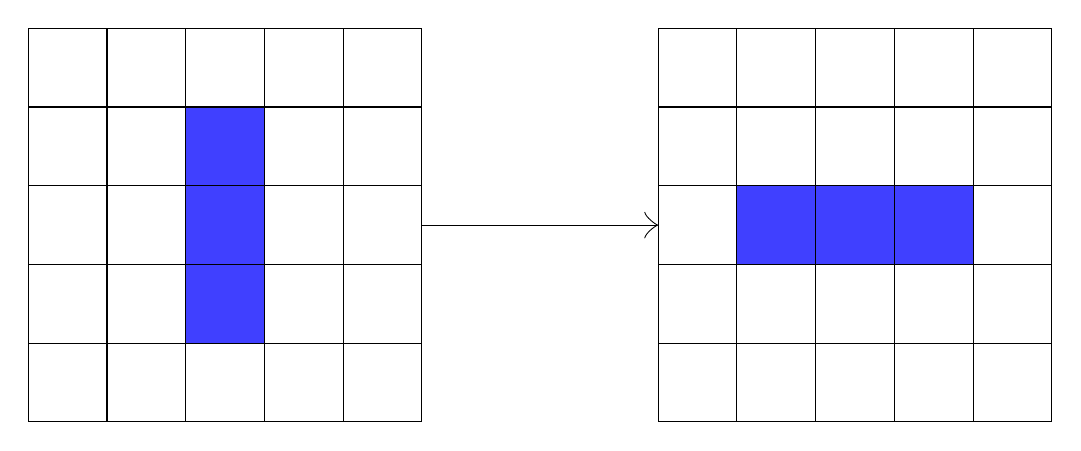
\begin{tikzpicture}
      \begin{scope}[xshift=-4cm]
        \grid{
          {0,0,0,0,0},
          {0,0,1,0,0},
          {0,0,1,0,0},
          {0,0,1,0,0},
          {0,0,0,0,0}}
        \node(arrstart) at (5,-2.5) {};
      \end{scope}
      \begin{scope}[xshift=4cm]
        \grid{
          {0,0,0,0,0},
          {0,0,0,0,0},
          {0,1,1,1,0},
          {0,0,0,0,0},
          {0,0,0,0,0}}
        \node(arrend) at (0,-2.5) {};
      \end{scope}
      \draw[-{Classical TikZ Rightarrow[length=5pt]}] (arrstart.center) -- (arrend.center);
    \end{tikzpicture}
    \subcaption{The pattern itself}
  \end{subfigure}\\
  \begin{subfigure}{\linewidth}
    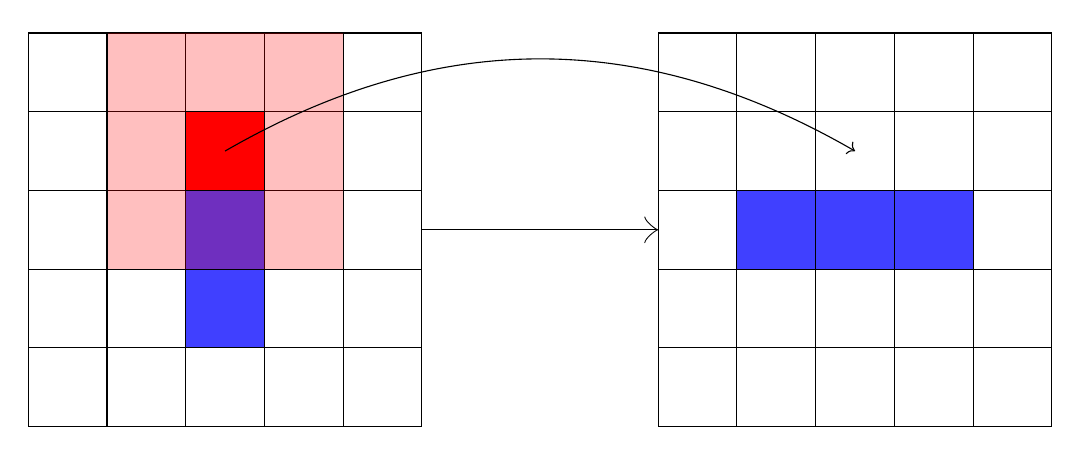
\begin{tikzpicture}
      \begin{scope}[xshift=-4cm]
        \grid{
          {0,0,0,0,0},
          {0,0,1,0,0},
          {0,0,1,0,0},
          {0,0,1,0,0},
          {0,0,0,0,0}}
        \node(arrstart) at (5,-2.5) {};
        \node(first) at (2.5,-1.5) {};
        \draw[fill=red,fill opacity=0.25] (1,0) rectangle ++(3,-3);
        \draw[fill=red] (2,-1) rectangle ++(1,-1);
      \end{scope}
      \begin{scope}[xshift=4cm]
        \grid{
          {0,0,0,0,0},
          {0,0,0,0,0},
          {0,1,1,1,0},
          {0,0,0,0,0},
          {0,0,0,0,0}}
        \node(arrend) at (0,-2.5) {};
        \node(second) at (2.5,-1.5) {};
      \end{scope}
      \draw[-{Classical TikZ Rightarrow[length=5pt]}] (arrstart.center) -- (arrend.center);
      \draw[->] (first.center) to[bend left] (second.center);
    \end{tikzpicture}
    \subcaption{With a live cell highlighted}
    \label{fig:GoLli}
  \end{subfigure}
  \begin{subfigure}{\linewidth}
    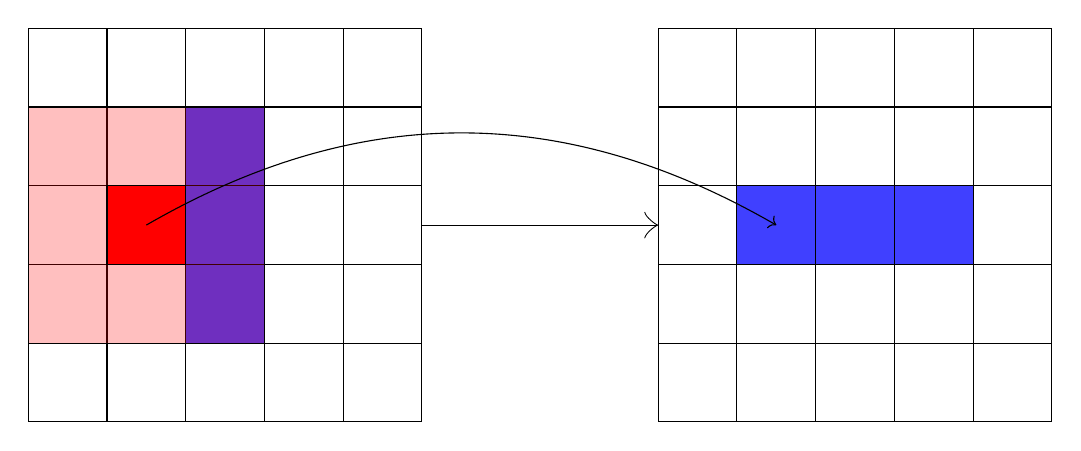
\begin{tikzpicture}
      \begin{scope}[xshift=-4cm]
        \grid{
          {0,0,0,0,0},
          {0,0,1,0,0},
          {0,0,1,0,0},
          {0,0,1,0,0},
          {0,0,0,0,0}}
        \node(arrstart) at (5,-2.5) {};
        \node(first) at (1.5,-2.5) {};
        \draw[fill=red,fill opacity=0.25] (0,-1) rectangle ++(3,-3);
        \draw[fill=red] (1,-2) rectangle ++(1,-1);
      \end{scope}
      \begin{scope}[xshift=4cm]
        \grid{
          {0,0,0,0,0},
          {0,0,0,0,0},
          {0,1,1,1,0},
          {0,0,0,0,0},
          {0,0,0,0,0}}
        \node(arrend) at (0,-2.5) {};
        \node(second) at (1.5,-2.5) {};
      \end{scope}
      \draw[-{Classical TikZ Rightarrow[length=5pt]}] (arrstart.center) -- (arrend.center);
      \draw[->] (first.center) to[bend left] (second.center);
    \end{tikzpicture}
    \subcaption{With a dead cell highlighted}
    \label{fig:GoLdi}
  \end{subfigure}
  \caption{Evolving a pattern by one generation using Conway's Game of Life}
  \label{fig:GoL}
\end{figure}

The effect of these rules can be seen in Figure~\ref{fig:GoL},
  which shows the effect of one application of the above rules on a small starting pattern.
Dead cells are drawn in white and live cells are drawn in blue.

To illustrate the rules more clearly, in Figure~\ref{fig:GoLli} one live cell is highlighted in red.
Its eight surrounding cells are highlighted in a lighter colour.
If we consider the middle cell, we can see that it is next to only one live cell,
  so by the Rule~\ref{itm:golao} above it turns into a dead cell.
Figure~\ref{fig:GoLdi} is similar, except that a dead cell is highlighted instead of a live cell.
This cell has three neighbouring live cells, so by Rule~\ref{itm:gold3} it becomes alive in the next generation.

\section{About Cabasa}
\label{sec:about}

Cabasa is an application for running \textbf{2D} cellular automata on (at the moment) a \textbf{finite} grid.
It aims to support any CA, unlike existing applications which can only support certain classes of CAs.
Do note that it does not aim to be particularly fast; if you want a very fast simulator, another application is probably better.

\chapter{Quickstart}
\label{chap:qstart}

To select a new rule, press the \menu{Control > Set Rule} menu item.
This opens a rule-selection dialog, where you can type a rule in or select a preexisting rule.
Cabasa comes with a set of predefined rules; to select one of these, use the menu item \menu{File > Open}.
In this example, we'll use the \texttt{life.alp} rule; it implements the \emph{Game of Life} rule described in Section~\ref{sec:whatisca}.
Selecting this rule and pressing the `Ok' button will make its contents appear in the dialog.
Press the \texttt{Set Rule} button to change the current rule to the rule which you have selected.

Now we can draw a pattern on the grid to use with this rule.
Select state \texttt{1} from the dropdown box at the top of the window marked `Current drawing state' (see screenshot, Figure~\ref{fig:mainwin}).
After this you should be able to draw patterns on the grid.
If you press the \keys{M} key, you can click and drag to move around; pressing \keys{D} gets you back to drawing mode.

To run the selected CA rule on your pattern, press the triangular `Play' button on the left of the screen;
  pressing it again should pause the evolution.
You should observe the pattern changing;
  this is due to the repeated application of the \emph{Game of Life} rules as described above.

\chapter{Getting Started}
\label{chap:gstart}

\section{User interface}
\label{sec:ui}

\begin{figure}[h]
  \centering
  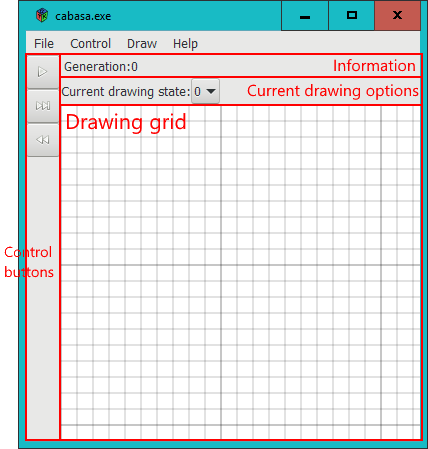
\includegraphics[scale=.8]{screenshot.png}
  \caption{Cabasa Main Window}
  \label{fig:mainwin}
\end{figure}

The main window, shown on Figure~\ref{fig:mainwin}, is composed of several parts.

The large grid in the middle shows the current state of the CA grid.
The user can draw on the grid, move around to show the rest of the grid, and use the currently loaded CA to evolve the pattern shown on the grid.

The information pane, just below the menu, shows various pieces of information about the current application state.
Currently it only shows the current generation,
  but it is expected that it will contain more information in future versions of Cabasa.

The drawing options pane, below the information pane, shows options related to drawing.
Again, there is currently only one thing shown here, but future versions may add more.
This pane will be disabled if drawing mode is not enabled.

\section{Drawing and Moving}
\label{sec:drming}

The application starts in \emph{drawing mode}.
In this mode, clicking and dragging on the grid changes the state of each cell the cursor passes over.

By default, the grid starts with all grid cells set to state 0 and the \emph{drawing state} also set to 0,
  so nothing happens when you try to draw on the grid.
However, by changing the selected state (next to the text `Current drawing state'), other states can be chosen.
For instance, if state 1 is selected, then clicking and dragging on the grid will change the cells under the cursor to state 1.
Note that the states are numbered starting from 0, not 1,
  so to select e.g.\ the second state you have declared you need to select state 1, not state 2.

Moving around the grid requires another mode, \emph{move mode}.
This mode can be selected from the \menu{Draw > Mode} menu, or by pressing the \keys{M} key.
You can get back to drawing mode by using the \menu{Draw} menu, or by pressing the \keys{D} key.
In this mode, clicking and dragging will not draw on the grid, but rather will move or pan around the grid.
Enabling this mode will also disable the `drawing options' pane.

In any mode, you can also zoom in and out using the mouse wheel.
Scroll up over a point to zoom in to that point, and scroll down to zoom out.

If you zoom out far enough, you will notice that the grid abruptly comes to an end at a certain point.
This is because the grid is finite.
However, the grid `wraps around' at its edges; that is, if you move off one edge of the grid, you reappear at the opposite edge.
For instance, the cell immediately above the topmost cell is considered to be the bottommost cell.

\section{Changing the Grid Size}
\label{sec:gridsize}

By default, Cabasa uses a $100 \times 100$ grid (unless this has been changed in the \hyperref[sec:sets]{Settings}.
This may be changed using the \menu{Edit > Change Grid Size} menu item, which launches a `Change Size' dialog.
This dialog may be used by entering the new size as $\text{width} \times \text{height}$,
  then pressing `OK'
  (or `Cancel' if you actually don't want to change the size).

\section{Selection and copying}
\label{sec:selcopy}

In addition to the two modes described above, there is also a mode for selecting parts of the grid.
This \emph{selection mode} may be accessed via the \menu{Draw > Mode} menu, like the other two modes,
  or with the \keys{S} hotkey.
In this mode, you may click and drag to select a portion of the grid (shown in green).
Click and drag again in a different part of the grid to make a new selection.
To clear the current selection, use the \hbox{\menu{Draw > Clear Selection}} menu item,
  or its hotkey \keys{\ctrl + K}.

Once you have selected part of a grid, you may \emph{copy} it into the \emph{clipboard},
  with the purpose of \emph{pasting} it back into another part of the grid.
To copy the selection, use the \menu{Edit > Copy} menu item.
To paste your selection back, press \menu{Edit > Paste};
  a brown overlay will then be shown at the location where your selection will be pasted.
Move your mouse, and then click on your document to paste your selection at the shown location.
The usual hotkeys \keys{\ctrl + C} and \keys{\ctrl + V} respectively may also be used.

\section{Changing the Rule}
\label{sec:chngrule}

The current CA can be changed using the \menu{Control > Set Rule} menu item.
This opens a window where you can type in a specification of a CA rule using the ALPACA specification language.

To accept a specification, press the `Set Rule' button at the bottom of the window.
This will interpret the specification and load it into the main window.
If the specification is invalid, it will show an error dialog instead.

After the rule is set, you will be able to draw patterns in this rule on the grid in the main window.
The set of states available for drawing through the `current drawing state' option will change to reflect the new rule.
Since the set of allowed states could have changed, the grid will be cleared after each rule change.

For more details on how to specify a CA, see Chapter~\ref{chap:speccas},
  but if you want to play around with a specification now then you can copy the following Game of Life specification into the `Set Rule' window:

\begin{verbatim}
state Dead  " "
  to Alive when 3 Alive and 5 Dead;
state Alive "*"
  to Dead when 4 Alive or 7 Dead.
\end{verbatim}

\section{Running CAs}
\label{sec:running}

A set of \emph{control buttons} can be seen on the left of the window.
These buttons are used to actually run the CA once a rule has been loaded and a pattern has been drawn.

To run one generation of the CA, use the middle button.
This operation is called \emph{stepping}.
You can repeatedly press this button to run the rules more than once.

The topmost button will repeatedly step the CA when it is pressed once.
This operation is generally referred to as \emph{running} the CA.
After this button has been pressed, the icon will change to a pause icon.
As this suggests, the button can be pressed again to pause the CA.
Pressing it again will allow the CA to be run again.

To adjust the rate of running, use the \menu{Control > Faster} and \menu{Control > Slower} menu items.
Alternatively, you may press the \keys{{+}} or \keys{-} keys respectively.
The current speed is shown at the top of the window as the delay between steps;
  that is, a smaller number indicates a faster speed.
Do note that Cabasa will not let you increase the speed below 100,
  since at these fast speeds Cabasa may crash when it attempts to calculate too quickly.

To reset the CA after you have run or stepped it, use the bottom `reset' button.
This button will restore the original state of the CA after you have pressed the `step' or `run' buttons.
If you haven't run the CA, then it doesn't do anything.

To clear the pattern, use the \menu{Draw > Clear} menu item.
This resets the generation, clears the pattern and moves the grid so that the top-left corner is displayed
  (as in the start of the program).

\section{Opening and Saving}
\label{sec:opsav}

Cabasa has the ability to open and save both rules and patterns.
This can be done through the \menu{File > Open} and \menu{File > Save As} menu items on the CA specification window and main window respectively.
\textit{Save} (as opposed to \textit{save as}) functionality has not yet been implemented, but will be implemented in a later version of Cabasa.

In more detail:

\begin{itemize}
\item To \textbf{save the current rule}, use the \menu{Control > Set Rule} menu item on the main window to open the CA selection window.
  Then press the \menu{File > Save As} menu item on the CA selection window to show a file selection dialog where you can save the current rule.
\item To \textbf{open a previously saved rule}, use the \menu{Control > Set Rule} menu item on the main window to open the CA selection window.
  Then press the \menu{File > Open} menu item on the CA selection window to show a file selection dialog where you can open a previously saved rule.
  After the rule has been opened, press the \textit{Set Rule} button at the bottom of the window to load it as the current rule.
\item To \textbf{save the current pattern}, use the \menu{File > Save As} menu item on the main window to show a file selection dialog where you can save the current pattern.
\item To \textbf{open a previously saved pattern}, use the \menu{File > Open} menu item on the main window to show a file selection dialog where you can open a previously saved pattern.
  If the pattern has been saved with a different rule to the rule currently active,
    a dialog box will be shown asking you if you want to switch rules.
\end{itemize}

\subsection{Finding rules}
\label{sec:findrs}

If Cabasa needs to find a previously-saved rule (as may occur when e.g.\ opening a saved pattern),
  it uses the following steps to find it:

\begin{enumerate}
\item Inspect the folder specified by the \texttt{User-defined rules directory} setting (see Section~\ref{sec:sets});
  use the rule if it is found in this folder.
\item Inspect the folder specified by the \texttt{Predefined rules directory} setting (see Section~\ref{sec:sets});
  use the rule if it is found in this folder.
\item The rule could not be found in any known folder; ask the user if they want to find it manually.
\end{enumerate}

\section{Settings}
\label{sec:sets}

Cabasa can be customised through the use of various settings.
These can be accessed through the \menu{File > Settings} menu item.
The following settings are currently supported:

\begin{description}
\item[Predefined rules directory]
  The directory in which sample rules are stored.
  (See Section~\ref{sec:findrs} for details.)
\item[User-defined rules directory]
  The directory in which user-defined rules are stored.
  (See Section~\ref{sec:findrs} for details.)
\item[Default grid size]
  A default grid size of $x \times y$ causes the default grid to have a size of $x$ columns by $y$ rows.
  Note that changing this setting does \textit{not} have any effect on the current grid;
    it only takes effect if a new grid is made.
\end{description}

\chapter{Specifying CAs}
\label{chap:speccas}

\section{Using ALPACA}
\label{sec:usalp}

ALPACA is a language created by Chris Pressey specifically for the specification of CAs.
Cabasa uses the ALPACA language to specify CAs; currently Cabasa supports ALPACA version 1.1.
Cabasa currently supports ALPACA version 1.1.

The reference manual for ALPACA version 1.1 is a very good guide for learning about the various features of ALPACA.
It is available at the following web address: \url{https://github.com/catseye/ALPACA/blob/0b2d57b8739dc240969c62c8e1cd13c1863770e0/doc/ALPACA.markdown}.
Cabasa should support all the features outlined in that manual
  \textbf{except} for the initial configuration, which is currently ignored.

Do note however that for technical reasons\footnotemark,
  the `examples' in the ALPACA manual are actually written in a format called `Falderal' and not plain ALPACA;
  the ALPACA translation can be found by reading the parts of the example which are after the \texttt{|} characters.
For instance, take this example from the manual:

\begin{verbatim}
| state Space " ";
| state Up "U"
|   to ^ when true;
| state Down "D"
|   to v when true
| begin
| DDD
| UUU
= -----
= UUU
= DDD
= -----
\end{verbatim}

For this example, the ALPACA which you would actually type is the following portion:

\begin{verbatim}
state Space " ";
state Up "U"
  to ^ when true;
state Down "D"
  to v when true
begin
DDD
UUU
\end{verbatim}

\footnotetext{In more detail: the `examples' are actually runnable tests containing an embedded description of the expected output as well.}

\section{Using ALPACA Stylesheets}
\label{sec:stys}

The \emph{ALPACA Stylesheets} format is a simple way to change the styling of a CA specified using ALPACA.
The format is documented at \url{https://github.com/catseye/ALPACA/blob/0b2d57b8739dc240969c62c8e1cd13c1863770e0/doc/ALPACA.markdown#alpaca-stylesheets-10}.

To open the ALPACA Stylesheets window, use the \menu{Draw > Edit Stylesheet} menu item.
This opens a window where you can edit the current stylesheet using the textbox in the middle of the screen,
  and then set it using the `Set Stylesheet' button at the bottom.
You can also use the \menu{File > Open} and \menu{File > Save As} menu items to open and save stylesheets respectively.

\appendix

\chapter{Sample Patterns and Rules}
\label{chap:samps}

Cabasa comes with a set of predefined example patterns and rules.
These are located in the default pattern and rule directories,
  so to access them you can simply use the relevant \menu{File > Open} menu items.

The predefined rules are:

\begin{description}
\item[life.alp] An ALPACA implementation of Conway's Game of Life
\item[bbrain.alp] An ALPACA implementation of \emph{Brian's Brain}, another well-known CA.
  This CA tends to explode chaotically, creating fascinating dynamic patterns.
\item[wireworld.alp] An ALPACA implementation of \emph{Wireworld}, a CA designed to simulate computer circuits.
  For more information on WireWorld, see \url{https://www.quinapalus.com/wires0.html}
\item[life.hs] A Haskell implementation of Conway's Game of Life.
  This in particular is a good template to start coding a CA in Haskell.
\item[langton.hs] A Haskell implementation of \textit{Langton's Ant}, a well-known CA simulating a moving `ant'.
  For more information on Langton's Ant, see \url{https://en.wikipedia.org/wiki/Langton%27s_ant}
\end{description}

The predefined patterns are:

\begin{description}
\item[pi.mcl \textnormal{and} r.mcl] The \emph{pi-heptomino} and \emph{r-pentomino}, two patterns which evolve in an interesting way when run using Conway's Game of Life.
\item[gates.mcl] The \textsc{and} and \textsc{or} logic gates in Wireworld.
\item[langton.mcl] An initial configuration for Langton's Ant.
\end{description}

\end{document}

% Local Variables:
% TeX-command-extra-options: "-shell-escape"
% End:
